\documentclass[10pt]{article}
\usepackage{amsmath,textcomp,amssymb,geometry,graphicx,enumerate,tikz,algorithm,algpseudocode,pifont}
\usetikzlibrary{calc}
\usetikzlibrary{datavisualization}
\usetikzlibrary{datavisualization.formats.functions}


\textheight=9in
\textwidth=7in
\topmargin=-.75in
\oddsidemargin=-0.25in
\evensidemargin=-0.25in

\usepackage{listings}
\lstnewenvironment{codeblock}
    {\lstset{language=Python,
      showspaces=false,
      showtabs=false,
      breaklines=true,
      mathescape=true,
      showstringspaces=false,
      breakatwhitespace=true,
      commentstyle=\textit,
      keywordstyle=\textbf,
      basicstyle=\ttfamily,
      escapechar=`,
      moredelim={**[is][{\color{RoyalBlue}}]{\^^M\\beginsol}{\^^M\\endsol}},
      moredelim={[is][{\color{RoyalBlue}}]{\^^M\\beginexp}{\^^M\\endexp}},
    }}
    {}

\begin{document}
	\section*{03/02/2016}
	\subsection*{Statistical Justification for Regression}
	\
	\begin{itemize}
		\item Typical model of reality:
			\begin{itemize}
				\item Samples come from unknown probability distribution $X_{i} \sim D$.
				\item y-values are sum of unknowns, non-random surface plus random noise: for all $X_{i}$,
					\begin{align*}
						y_{i} = f(X_{i}) + \epsilon_{i}
					\end{align*}
			\end{itemize}
		\item Goal of regression: find $h$ that estimates f.
		\item Ideal approach: choose $h(x) = E_{y}[Y | X=x]$
	\end{itemize} 
	
	\subsection*{Least-squares Regression from Max Likelihood}
	\
	\begin{itemize}
		\item Suppose $\epsilon_{i} \sim \mathcal{N}(0, \sigma^{2})$; then $y_{i}|X_{i} \sim \mathcal{N}(f(X_{i}), \sigma^{2})$.
		\item Recall that log likelihood for normal distribution is,
			\begin{align*}
				ln P(y_{i}) &= - \frac{|y_{i} - \mu|^{2}}{2\sigma^{2}} - constant \ \ \ \ \ \ \Leftarrow \mu = f(X_{i})\\
				ln(P(y_{1})P(y_{2}) \dots P(y_{n})) &= ln P(y_{1}) + ln P(y_{2}) + \dots + ln P(y_{n})\\
			\end{align*}
		\item Takeaway: If you apply the principle of max likelihood to linear regression with an input model that assumes gaussian noise $\Rightarrow$ find $f$ by least-squares. 
	\end{itemize}
	
	\subsection*{Empirical Risk}
	\
	\begin{itemize}
		\item The \underline{risk} for hypothesis $h$ is the expected loss $R(h) = E[L]$ over all $X, Y$.
		\item Discriminative model: we don't know $X'$s distribution D. How can we minimize the risk?
		\item \underline{Empirical distribution}: A discrete probability that is the sample set, with each sample equally likely.
		\item \underline{Empirical risk}: expected loss over empirical distribution $\hat{R}(h) = \frac{1}{n} \sum_{i=1}^{n} L(h(X_{i}), y_{i}))$.
		\item Takeaway: this is why we minimize the sum of loss functions.
	\end{itemize}
	
	\subsection*{Logistic regression from Max Likelihood}
	\
	\begin{itemize}
		\item If we accept the logistic regression function, what cost function should we use?
		\item Given arbitrary sample $x$, write probability it is in (not in) the class: (fictitious dimension: x ends w/1; $w$ ends w/$\alpha$).
			\begin{align*}
				P(y=1|x;w) &= h(x;w) \ \ \ \ \ \ \ \ \Leftarrow h(x;w) = s(w^{T}x)\\
				P(y=0|x;w) &= 1 - h(x;w)\\
			\end{align*}
		\item Combine these 2 facts into 1 expression:
			\begin{align*}
				P(y|x;w) = h(x)^{y}(1 - h(x))^{1-y}\\
			\end{align*}
		
		\item Likelihood is,
			\begin{align*}
				L(w; x_{1}, \dots, x_{n}) &= \prod_{i=1}^{n} P(y_{i}|X_{i};w)\\
				l(w) = ln L(w) &= \sum_{i=1}^{n} ln P(y_{i}|X_{i};w)\\
				&= \sum (y_{i}ln h(X_{i}) + (1-y_{i})ln(1-h(X_{i})))
			\end{align*}
		\item which is negated logistic cost function J(w).
	\end{itemize}
	
	\subsection*{The Bias-variance Decomposition}
	\
	\begin{itemize}
		\item There are 2 sources of error in a hypothesis h:
			\begin{itemize}
				\item \underline{bias}: error due to inability of hypothesis $h$ to fit $f$ perfectly. e.g. fitting quadratic $f$ with a linear $\ell$.
				\item \underline{variance}: error due to fitting random noise in data. e.g. we fit linear $f$ with a linear $h$, yes $h \neq f$.
			\end{itemize}
		\item Model: generate samples $X_{1} \dots X_{n}$ from some distribution $D$. Values $y_{i} = f(X_{i}) + \epsilon_{i}$. Fit hypothesis $h$ to $X, y$.
		\item Now $h$ is a random variable; i.e. its weights are random.
		\item Consider an arbitrary point $z \in \mathbb{R}^{d}$ (not necessarily a sample!) and $\gamma = f(z) + \epsilon$.
		\item Note: $\text{E}[\gamma] = f(z) ; \text{Var}(\gamma) = \text{Var}(\epsilon)$;
		\item Risk function when loss is squared error:
		\item Here we are taking the expectation over all possible training sets $X,y$ and values of $\gamma$.
			\begin{align*}
				R(h) &= E[L(h(z), \gamma)]\\
					&= E[(h(z) - \gamma)^{2}]\\
					&= E[h(z)^{2}] + E[\gamma^{2}] - 2E[\gamma h(z)]\\
					&= \text{Var}(h(z)) + E[h(z)]^{2} + \text{Var}(\gamma) + E[\gamma]^{2} - 2E[\gamma]E[h(z)]\\
					&= (E[h(z)] - E[\gamma])^{2} + \text{Var}(h(z)) + \text{Var}(\gamma)\\
					&= E[h(z) - f(z)]^{2} + \text{Var}(h(z)) + \text{Var}(\epsilon)\\
			\end{align*}
			\begin{itemize}
				\item We take expectation over possible training sets, $X, y$ and values of $\gamma$.
				\item $E[h(z) - f(z)]^{2}$: is square of the bias of method.
				\item $\text{Var}(h(z))$: variance of method.
				\item $\text{Var}(\epsilon)$: irreducible error (comes from test point not from training).
			\end{itemize}
			
			\item This is point-wise version. Mean version: Let $z \sim D$ be random variable; take expectation of the squares bias, variance over $z$
				\begin{center}
					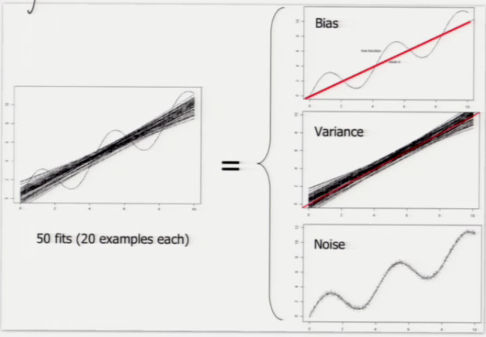
\includegraphics[scale=0.5]{../images/noise}
				\end{center}
				\begin{itemize}
					\item Under-fitting: too much bias.
					\item Over-fitting caused by too much variance. 
				\end{itemize}
			\item Training error reflects bias but not variance; test error reflects both.
			\item For many distributions, variance $\rightarrow$ 0 as $n \rightarrow \infty$.
			\item If $h$ can fit $f$ exactly, for many distributions bias $\rightarrow 0$ as $n \rightarrow \infty$.
			\item If $h$ cannot fit $f$ well, bias is large at "most" points.
			\item Adding a good feature reduces bias; adding a bad feature rarely increases it.
			\item Adding a feature usually increases variance.
			\item Cannot reduce irreducible error.
			\item Noise in test set affects only var($\epsilon$); noise in training set affects only bias and Var(h).
			\item For real-world data, $f$ is rarely knowable (and noise model might be wrong).
			\item But we can test learning algorithms by choosing $f$ and making synthetic data.
				\begin{center}
					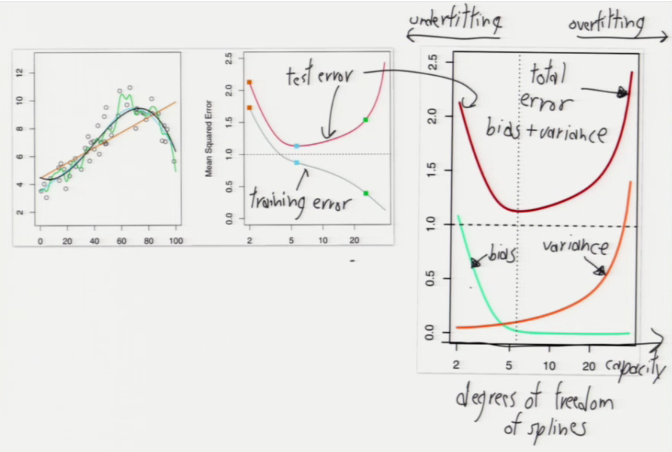
\includegraphics[scale=0.5]{../images/errorvsbias}
				\end{center}
			\item Example: Least-Squares Linear Regression:
				\begin{itemize}
					\item No fictitious dimension.
					\item Model: $f(z) = v^{T}z$.
					\item Let $e$ be a noise n-vector $e\sim \mathcal{N}(0, \sigma^{2})$.
					\item Training values: $y = Xv + e$. Input to regression algorithm are $y, X$.
					\item Linear regression computes weights:
						\begin{align*}
							w = X^{+}y = X^{+}(Xv + e) = v + X^{+}e
						\end{align*}
					\item Bias is,
						\begin{align*}
							E[h(z) - f(z)] = E[w^{T}z - v^{T}z] = E[z^{T}X^{+}e] = z^{T}X^{+}E[e] = 0
						\end{align*}
					\item Warning: This does not mean $h(z) - f(z)$ is everywhere 0. Sometimes positive, sometimes negative, mean over training sets is 0.
					\item Variance is,
						\begin{align*}
							\text{Var}(h(z)) &= \text{Var}(w^{T}z) = \text{Var}(z^{T}w)\\ 
							&= \text{Var}(z^{T}(v + X^{+}e)\\
							&= \text{Var}(z^{T}v + z^{T}X^{+}e))\\ 
							&= \text{Var}(z^{T}X^{+}e)\\
							&= \sigma^{2} |z^{T}X^{+}|^{2}\\
							&= \sigma^{2} |z^{T}(X^{T}X)^{-1}X^{T})|^{2}\\
							&= \sigma^{2} z^{T}(X^{T}X)^{-1}X^{T}X(X^{T}X)^{-1}z\\
							&= \sigma^{2}z^{T}(X^{+}X)^{-1}z
						\end{align*}
					\item If choose coordinate system so $E[X] = 0$ it simplifies to $\approx \sigma^{2}\frac{d}{n}$.
					\item Takeaways: Bias can be zero when hypothesis function can fit the real one. Variance portion of RSS (overfitting) decreases as $\frac{1}{n}$, increases as $d$.
				\end{itemize}
	\end{itemize}	
\end{document}
